\documentclass[tikz,border=5pt]{standalone}
\usepackage[utf8]{inputenc}
\usepackage[T1]{fontenc}
\usepackage{lmodern,amsmath,amssymb}
\usepackage[american]{circuitikz}
\usepackage{pgfplots}
\pgfplotsset{compat=1.18}
\usetikzlibrary{circuits.logic.US,positioning,calc,arrows.meta,patterns,shapes.geometric}
\definecolor{Primary}{HTML}{1F77B4}
\begin{document}
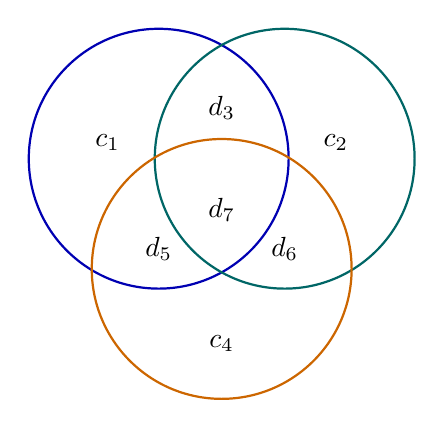
\begin{tikzpicture}[thick]
\draw[blue!70!black](-.8,.5)circle(1.65);\draw[teal!80!black](.8,.5)circle(1.65);\draw[orange!80!black](0,-.9)circle(1.65);
\node at(-1.45,.7){$c_1$};\node at(1.45,.7){$c_2$};\node at(0,-1.85){$c_4$};
\node at(0,1.15){$d_3$};\node at(-.8,-.65){$d_5$};\node at(.8,-.65){$d_6$};\node at(0,-.15){$d_7$};

\end{tikzpicture}
\end{document}
